
\begin{frame}{One Column}
    \begin{enumerate}
      \item
    \end{enumerate}
    \begin{equation}\label{l}
        \int_0^\infty f(x)dx = x^2\sqrt{x}
    \end{equation}
\end{frame}


\begin{frame}[t,fragile]{Two-Column}
    \begin{columns}[t]
        \column{0.6\textwidth}
        \begin{itemize}
            \item
        \end{itemize}
        \column{0.4\textwidth}
            \begin{figure}
              \centering
              %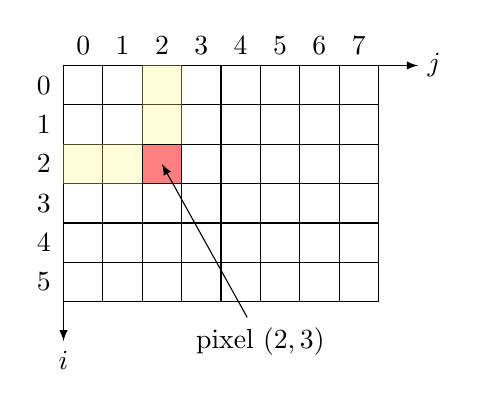
\begin{tikzpicture}[scale=0.5]
	\foreach \i in {0,1,...,6}
	{
		\draw (0,\i) -- ++(8,0);
	}
	\foreach \i in {0,1,...,5}
	{
		\node at (-0.5, 5.5 - \i) {$\i$};
	}	
	\foreach \j in {0,1,...,8}
	{
		\draw (\j,0) -- ++(0,6);
	}
	\foreach \j in {0,1,...,7}
	{
		\node at (\j + 0.5, 6.5) {$\j$};
	}		
	\draw[-latex] (0,6) -- ++(0,-7) node[anchor=north] {$i$};		
	\draw[-latex] (0,6) -- ++(9,0) node[anchor=west] {$j$};

    \pause
    \draw [draw=none, fill=yellow!50, opacity=0.3] (0,3) rectangle (3,4);
    \draw [draw=none, fill=yellow!50, opacity=0.3] (2,3) rectangle (3,6);
    \draw[fill=red!50] (2,3) rectangle ++(1,1);
    \node (a) at  (5,-1) {pixel $(2,3)$};
    \draw[-latex] (a) -- (2.5,3.5);
	
\end{tikzpicture} 
              \caption{}
            \end{figure}
    \end{columns}

\end{frame}

\begin{frame}[fragile]{Two-Column Code}
    \begin{columns}[t]
    \column[t]{0.5\textwidth}
           \begin{lstlisting}[caption=A Grayscale Image, language=Python, escapechar=\@]
    %matplotlib inline

            \end{lstlisting}
    \column[t]{0.5\textwidth}
           \begin{lstlisting}[caption=A Color Image,language=Python, escapechar=\@]
    %matplotlib inline

             \end{lstlisting}
    \end{columns}
\end{frame}

\begin{frame}[t, fragile]{One-Column Code}
    \begin{lstlisting}[caption=Displaying  Image Properties, language=Python, escapechar=\@]
%matplotlib inline
import cv2 as cv
import matplotlib.pyplot as plt
img = cv.imread('../images/hugh.jpg', cv.IMREAD_COLOR)
img = cv.cvtColor(img, cv.COLOR_BGR2RGB)
fig, ax = plt.subplots()
ax.imshow(img)
ax.set_title('Image')
plt.show()
@\fillblank{print(img.shape)}@
@\fillblank{print(img.size)}@
@\fillblank{print(img.dtype)}@
    \end{lstlisting}
\end{frame} 


% Four Pictures
\begin{frame}{Examples of Effect of Kernel Choices}
    \begin{figure}
        \centering
        \begin{subfigure}[b]{0.35\textwidth}
            \includegraphics[width=\textwidth]{./figures/sigiriya.jpg}
            \caption{Original}
            \label{sfi:sigiriya_original}
        \end{subfigure}
        \hspace{1cm}
        \begin{subfigure}[b]{0.35\textwidth}
            \includegraphics[width=\textwidth]{./figures/sigiriya_averaged.jpg}
            \caption{Avegaging}
            \label{sfi:sigiriya_averaged}
        \end{subfigure}\\
        \centering
        \begin{subfigure}[b]{0.35\textwidth}
            \includegraphics[width=\textwidth]{./figures/sigiriya_sobel_horizontal.jpg}
            \caption{Sobel horizontal}
            \label{sfi:sigiriya_sobel_horizontal}
        \end{subfigure}
        \hspace{1cm}
        \begin{subfigure}[b]{0.35\textwidth}
            \includegraphics[width=\textwidth]{./figures/sigiriya_sobel_vertical.jpg}
            \caption{Sobel vertical}
            \label{sfi:sigiriya_averaged}
        \end{subfigure}
        \caption{Effect of kernels.}\label{fi:effect_of_kernels}
    \end{figure}
\end{frame}